\documentclass[12pt]{article}
\usepackage{amssymb,amsmath,latexsym}

\usepackage{graphicx}
\usepackage{epstopdf}

% Page length commands go here in the preamble
\setlength{\oddsidemargin}{-0.25in} % Left margin of 1 in + 0 in = 1 in
\setlength{\textwidth}{7in}   % Right margin of 8.5 in - 1 in - 6.5 in = 1 in
\setlength{\topmargin}{-.75in}  % Top margin of 2 in -0.75 in = 1 in
\setlength{\textheight}{9.2in}  % Lower margin of 11 in - 9 in - 1 in = 1 in

\newtheorem{theorem}{Theorem}
\newtheorem{definition}{Definition}

\renewcommand{\baselinestretch}{1.5} % 1.5 denotes double spacing. Changing it will change the spacing

\setlength{\parindent}{0in} 
\begin{document}
\title{A Sample \LaTeX \;Article}
\author{John Doe}
\date{\today}
\maketitle
\abstract{This a sample \LaTeX document that explains some of the \LaTeX commands}

\section{Introduction}
\LaTeX \; is a markup language designed and implemented by \textbf{Leslie Lamport}, based on \textbf{Donald E. Knuth}'s typesetting language \TeX.  The markup in the source file of a \LaTeX \; document my appear somewhat challenging, but the compiled result of the document is certainly a pleasing rendering of the mark-up material.\\


%\begin{figure}[!htb]
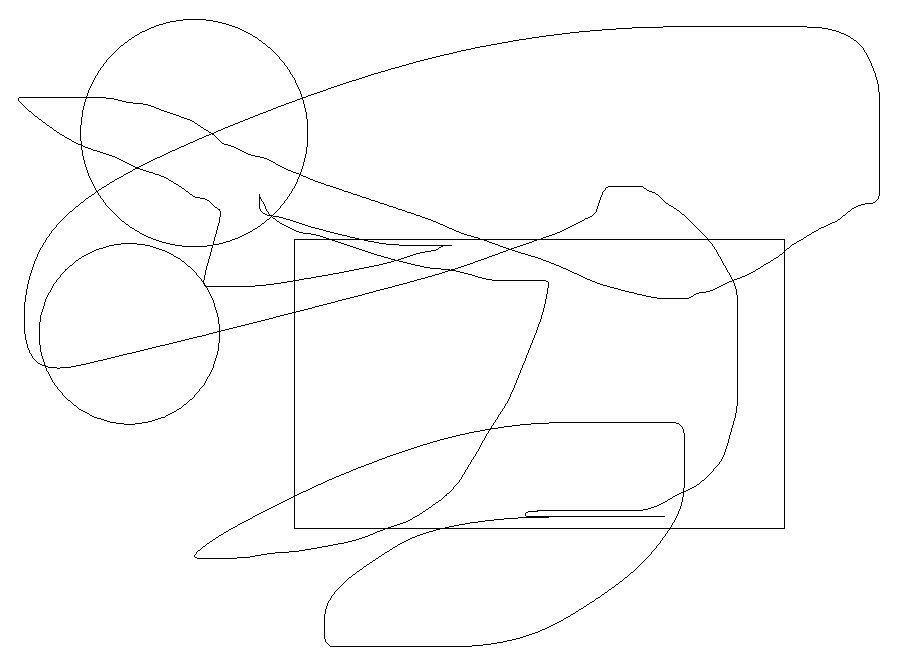
\includegraphics{test-eps.eps}
%\end{figure}


\section{Typing Text}
The following keys are used to type text in a \LaTeX \; source file: 
\begin{center}
   \begin{verbatim}
         a-z  A-Z  0-9
         +  =  *  /  ( )  [ ]
   \end{verbatim}
\end{center}
You may also use the following punctuation marks:
\begin{center}
   \begin{verbatim}
     ,  ;  .  ?  !  :  `  '  -
   \end{verbatim}
\end{center}
and the spacebar, and the Return (or Enter) key.\\


\section{References}
Michael Downes \emph{Short Math Guide for \LaTeX}, AMS, 2002\\[0.2in]
George Gratzer, \emph{First Steps in \LaTeX}, Springer-Verlag, New York, 1999\\[0.2in]


\end{document}
